\section{GONIOMETRIE} \label{goniometrie}
\hypertarget{goniometrie}{}

\subsection{Goniometrische getallen van een hoek} \label{goniometrische_getallen}
\hypertarget{goniometrische_getallen}{}

\subsubsection{In een rechthoekige driehoek} \label{rechthoekige_driehoek}
\hypertarget{rechthoekige_driehoek}{}

\begin{center}
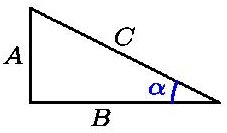
\includegraphics{rechtdriehoek.jpg}
\end{center}
\begin{eqnarray*}
\sin\alpha&=&\ds\Frac{A}{C}\\
\cos\alpha&=&\ds\Frac{B}{C}\\
\mbox{tg}\:\alpha&=&\ds\Frac{\sin\alpha}{\cos\alpha}=\ds\Frac{A}{B}\\
\mbox{cotg}\:\alpha&=&\ds\Frac{1}{\mbox{tg}\alpha}=\ds\Frac{B}{A}
\end{eqnarray*}

\subsubsection{De goniometrische cirkel} \label{goniometrische_cirkel}
\hypertarget{goniometrische_cirkel}{}

\begin{center}
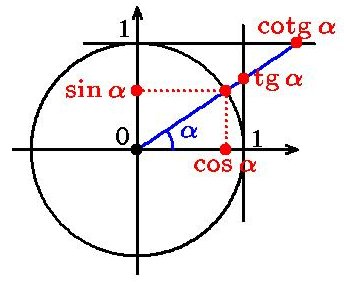
\includegraphics{goncirkel.jpg}
\end{center}

\subsubsection{Formules} \label{goniometrische_formules}
\hypertarget{goniometrische_formules}{}

\begin{itemize}
\item \textcolor{green}{Grondformule en afgeleide formules}
\begin{eqnarray*}
\ds\Frac{1}{\sin\alpha} & = & \mbox{cosec}\alpha\\
\ds\Frac{1}{\cos\alpha} & = & \mbox{sec}\alpha\\
\cos^2\alpha+\sin^2\alpha&=&1\\
1+\:\mbox{tg}^2\alpha &=&\:\mbox{sec}^2\alpha\\
1+\:\mbox{cotg}^2\alpha&=&\:\mbox{cosec}^2\alpha
\end{eqnarray*}
\item \textcolor{green}{\hypertarget{verwante_hoeken}{Verwante hoeken}}\label{verwante hoeken}
	\begin{itemize}%verwante hoeken
	\item[*] Tegengestelde hoeken ($\alpha$ en $-\alpha$)
	\begin{eqnarray*}
	\sin(-\alpha)& =&-\sin\alpha\\
	\cos(-\alpha)&=&\cos\alpha\\
	\mbox{tg}\:(-\alpha)&=&-\:\mbox{tg}\:\alpha\\
	\mbox{cotg}\:(-\alpha)&=&-\:\mbox{cotg}\:\alpha
	\end{eqnarray*}
	\item[*] Supplementaire hoeken ($\alpha$ en $\pi-\alpha$)
	\begin{eqnarray*}
	\sin(\pi-\alpha)& =&\sin\alpha\\
	\cos(\pi-\alpha)&=&-\cos\alpha\\
	\mbox{tg}\:(\pi-\alpha)&=&-\:\mbox{tg}\:\alpha\\
	\mbox{cotg}\:(\pi-\alpha)&=&-\:\mbox{cotg}\:\alpha
	\end{eqnarray*}
	\item[*] Complementaire hoeken ($\alpha$ en $\ds\Frac{\pi}{2}-\alpha$)
	\begin{eqnarray*}
	\sin(\ds\Frac{\pi}{2}-\alpha)& =&\cos\alpha\\
	\cos(\ds\Frac{\pi}{2}-\alpha)&=&\sin\alpha\\
	\mbox{tg}\:(\ds\Frac{\pi}{2}-\alpha)&=&\:\mbox{cotg}\:\alpha\\
	\mbox{cotg}\:(\ds\Frac{\pi}{2}-\alpha)&=&\:\mbox{tg}\:\alpha
	\end{eqnarray*}
	\item[*] Antisupplementaire hoeken ($\alpha$ en $\pi+\alpha$)
	\begin{eqnarray*}
	\sin(\pi+\alpha)& =&-\sin\alpha\\
	\cos(\pi+\alpha)&=&-\cos\alpha\\
	\mbox{tg}\:(\pi+\alpha)&=&\:\mbox{tg}\:\alpha\\
	\mbox{cotg}\:(\pi+\alpha)&=&\:\mbox{cotg}\:\alpha
	\end{eqnarray*}
	\item[*] Anticomplementaire hoeken ($\alpha$ en $\ds\Frac{\pi}{2}+\alpha$)
	\begin{eqnarray*}
	\sin(\ds\Frac{\pi}{2}+\alpha)& =&\cos\alpha\\
	\cos(\ds\Frac{\pi}{2}+\alpha)&=&-\sin\alpha\\
	\mbox{tg}\:(\ds\Frac{\pi}{2}+\alpha)&=&-\:\mbox{cotg}\:\alpha\\
	\mbox{cotg}\:(\ds\Frac{\pi}{2}+\alpha)&=&-\:\mbox{tg}\:\alpha
	\end{eqnarray*}
	\end{itemize}%verwante hoeken
\item \textcolor{green}{\hypertarget{som-en_verschilformules}{Som- en verschilformules}}\label{som-en_verschilformules}
\begin{eqnarray*}
\cos(\alpha-\beta)&=&\cos\alpha\,\cos\beta+\sin\alpha\,\sin\beta\\
\cos(\alpha+\beta)&=&\cos\alpha\,\cos\beta-\sin\alpha\,\sin\beta\\	
\sin(\alpha+\beta)&=&\sin\alpha\,\cos\beta+\cos\alpha\,\sin\beta\\
\sin(\alpha-\beta)&=&\sin\alpha\,\cos\beta-\cos\alpha\,\sin\beta\\
\mbox{tg}\:(\alpha+\beta)&=&\ds\Frac{\mbox{tg}\:\alpha+\:\mbox{tg}\:\beta}{1-	\:\mbox{tg}\:\alpha\:\mbox{tg}\:\beta}\\
\mbox{tg}\:(\alpha-\beta)&=&\ds\Frac{\mbox{tg}\:\alpha-	\:\mbox{tg}\:\beta}{1+	\:\mbox{tg}\:\alpha\:\mbox{tg}\:\beta}
\end{eqnarray*}
\item \textcolor{green}{\hypertarget{simpson}{Formules van Simpson}}\label{simpson}
\begin{eqnarray*}
\sin\alpha+\sin\beta&=&2\sin\ds\Frac{\alpha+\beta}{2}\,\cos\ds\Frac{\alpha-\beta}{2}\\
\sin\alpha-\sin\beta&=&2\cos\ds\Frac{\alpha+\beta}{2}\,\sin\ds\Frac{\alpha-\beta}{2}\\
\cos\alpha+\cos\beta&=&2\cos\ds\Frac{\alpha+\beta}{2}\,\cos\ds\Frac{\alpha-\beta}{2}\\
\cos\alpha-\cos\beta&=&-2\sin\ds\Frac{\alpha+\beta}{2}\,\sin\ds\Frac{\alpha-\beta}{2}\\
\end{eqnarray*}
\item \textcolor{green}{\hypertarget{dubbele_hoek}{Formules voor de dubbele hoek}}\label{dubbele_hoek}
\begin{eqnarray*}
\sin(2\alpha)&=&2\sin\alpha\,\cos\alpha\\
\cos(2\alpha)&=&\cos^2\alpha - \sin^2\alpha\\
\mbox{tg}(2\alpha)&=&\ds\Frac{2\:\mbox{tg}\:\alpha}{1-\:\mbox{tg}^2\alpha}
\end{eqnarray*}
\item \textcolor{green}{\hypertarget{t-formules}{t-formules}}\label{t-formules}\newline
Stel $\mbox{tg}\Frac{\alpha}{2}=t$, dan kunnen we $\sin\alpha, \cos\alpha$ en 	$\mbox{tg}\,\alpha$ schrijven in functie van $t$.
\begin{eqnarray*}
\sin\alpha&=&\Frac{2t}{1+t^2}\\
\cos\alpha&=&\Frac{1-t^2}{1+t^2}\\
\mbox{tg}\,\alpha&=&\Frac{2t}{1-t^2}
\end{eqnarray*}
\end{itemize}

\subsubsection{Oplossen van driehoeken} \label{oplossen_driehoeken}
\hypertarget{oplossen_driehoeken}{}
	\begin{itemize}%oplossen van drhn
	\item \textcolor{green}{Rechthoekige driehoeken}
		\begin{itemize}%rechthoekige drhn
		\item[*]De stelling van Pythagoras:
		\[C^2=A^2+B^2\]
		\end{itemize}%rechthoekige drhn
	\item \textcolor{green}{Willekeurige driehoeken}\newline
		%\docLink[tekening]{driehoek.jpg}{\includegraphics{tekening.gif}}
                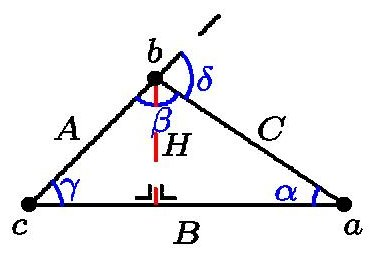
\includegraphics{driehoek.jpg}
		\begin{itemize}%willekeurige drhn
		\item[*] De \hypertarget{sinusregel}{{\bf sinusregel}}:\label{sinusregel}
		\[\ds\Frac{A}{\sin\alpha}=\ds\Frac{B}{\sin\beta}=\ds\Frac{C}{\sin\gamma}=2R\]
		met $R$ de straal van de omgeschreven cirkel.\newline
		\item[*] De \hypertarget{cosinusregel}{{\bf cosinusregel}}:\label{cosinusregel}
		\begin{eqnarray*}
		A^2&=&B^2+C^2-2BC\cos\alpha\\
		B^2&=&A^2+C^2-2AC\cos\beta\\
		C^2&=&A^2+B^2-2AB\cos\gamma
		\end{eqnarray*}
		\end{itemize}%willekeurige drhn
	\end{itemize}%oplossen van drhn


\subsection{Goniometrische functies}

Zie Sectie~\ref{subsubsec:goniometrische_functies} op pagina~\pageref{subsubsec:goniometrische_functies}.


% Dit werk is gelicenseerd onder een Creative Commons
% Naamsvermelding-GelijkDelen 3.0 Unported.
% Bezoek http://creativecommons.org/licenses/by-sa/3.0/ om een kopie te zien 
% van de licentie of stuur een brief naar Creative Commons, 444 Castro Street, 
% Suite 900, Mountain View, California, 94041, USA.